% Reporte: Análisis estático de seguridad con CodeQL en hindama-backend
% Compilar con: tectonic main.tex   (XeLaTeX; usa Arial y Menlo del sistema)
\documentclass[11pt,a4paper]{article}

% ---------- Idioma y fuentes ----------
\usepackage{fontspec}
\usepackage[spanish,es-noquoting,es-noshorthands,es-nodecimaldot,es-tabla]{babel}
\setmainfont{Arial}
\setmonofont{Menlo}[Scale=0.85]

% ---------- Página ----------
\usepackage[a4paper,top=2.5cm,bottom=2.5cm,left=2.5cm,right=2.5cm]{geometry}
\usepackage{fancyhdr}
\pagestyle{fancy}
\fancyhf{}
\fancyfoot[L]{\small\thepage}
\fancyfoot[R]{\small\color{gris}CodeQL en hindama-backend}
\renewcommand{\headrulewidth}{0pt}
\fancypagestyle{plain}{\fancyhf{}\fancyfoot[L]{\small\thepage}\renewcommand{\headrulewidth}{0pt}}
\setlength{\parindent}{0pt}
\setlength{\parskip}{0.55em}
\linespread{1.12}

% ---------- Paquetes ----------
\usepackage{xcolor}
\usepackage{graphicx}
\usepackage{tikz}
\usepackage{booktabs}
\usepackage{tabularx}
\usepackage{array}
\usepackage{float}
\usepackage[font=small,labelfont=bf,textfont=it]{caption}
\usepackage{enumitem}
\usepackage{titlesec}
\usepackage{listings}
\usepackage{hyperref}

\definecolor{azul}{HTML}{1F4E79}
\definecolor{azulclaro}{HTML}{2E75B6}
\definecolor{gris}{HTML}{6B6B6B}
\definecolor{fondo}{HTML}{F4F6F8}
\definecolor{borde}{HTML}{D0D7DE}
\definecolor{cadena}{HTML}{0A6B2E}
\definecolor{comentario}{HTML}{6B6B6B}
\definecolor{clave}{HTML}{8A2BE2}

\hypersetup{colorlinks=true,linkcolor=azul,urlcolor=azulclaro,
  pdftitle={Análisis estático de seguridad con CodeQL},
  pdfauthor={Selvas De León Luis Antonio; Pérez Aguilera Luis Angel}}

\titleformat{\section}{\Large\bfseries\color{azul}}{\thesection.}{0.5em}{}
\titleformat{\subsection}{\large\bfseries\color{azulclaro}}{\thesubsection}{0.5em}{}
\titlespacing*{\section}{0pt}{1.4em}{0.6em}
\titlespacing*{\subsection}{0pt}{1.1em}{0.4em}

\setlist{itemsep=0.25em,topsep=0.3em}

% ---------- Código ----------
\lstdefinelanguage{QL}{
  morekeywords={import,predicate,from,where,select,and,or,not,instanceof,result,exists,class,extends,string,int},
  sensitive=true,
  morecomment=[l]{//},
  morecomment=[s]{/*}{*/},
  morestring=[b]",
}
\lstdefinelanguage{yaml}{
  morekeywords={name,queries,uses,paths-ignore,on,push,pull_request,branches,workflow_dispatch,permissions,jobs,steps,with,runs-on},
  sensitive=true,
  morecomment=[l]{\#},
  morestring=[b]",
}
\lstset{
  basicstyle=\ttfamily\small,
  backgroundcolor=\color{fondo},
  frame=single, rulecolor=\color{borde}, framesep=6pt, xleftmargin=6pt, xrightmargin=6pt,
  keywordstyle=\color{clave}\bfseries,
  stringstyle=\color{cadena},
  commentstyle=\color{comentario}\itshape,
  numbers=left, numberstyle=\tiny\color{gris}, numbersep=10pt,
  breaklines=true, breakatwhitespace=false, columns=fullflexible, keepspaces=true,
  showstringspaces=false, tabsize=2, upquote=true,
  aboveskip=0.8em, belowskip=0.8em,
  captionpos=b,
}
\renewcommand{\lstlistingname}{Listado}
\renewcommand{\lstlistlistingname}{Listados}

\newcommand{\cod}[1]{\texttt{#1}}
\newcommand{\captura}[3][0.95]{%
  \begin{figure}[H]\centering
    \includegraphics[width=#1\linewidth]{img/#2}
    \caption{#3}
  \end{figure}}

\newcolumntype{L}{>{\raggedright\arraybackslash}X}

\begin{document}

% ======================= PORTADA =======================
\begin{titlepage}
\thispagestyle{empty}
\begin{tikzpicture}[remember picture,overlay]
  \node[anchor=north east,inner sep=0] at (current page.north east)
    {
\includegraphics[width=0.5\paperwidth,height=\paperheight]{img/ondas.png}};
\end{tikzpicture}
\fontsize{12}{18}\selectfont
\vspace*{0.4cm}

\includegraphics[width=4.1cm]{img/logo-upchiapas.png}

\vspace{1.3cm}
\textbf{Universidad Politécnica de Chiapas}\\
\hspace*{1.3cm}\textbf{Ingeniería en software}

\vspace{1.4cm}
\textbf{Materia:} Seguridad Informática

\vspace{1.0cm}
\textbf{Actividad:}\\
Análisis estático de seguridad con CodeQL:\\
detección y eliminación de variantes de\\
inyección SQL en hindama-backend

\vspace{1.4cm}
\textbf{Estudiantes:}\\
Selvas De León Luis Antonio\\
Pérez Aguilera Luis Angel

\vspace{1.0cm}
\textbf{Matrículas:}\\
243472\\
243757

\vspace{1.0cm}
\textbf{Fecha de entrega:}\\
18 / Noviembre / 2026
\end{titlepage}

% ======================= ÍNDICE =======================
\tableofcontents
\newpage

% ======================= 1 =======================
\section{Introducción}

\textbf{CodeQL} es el motor de análisis semántico de código de GitHub. Convierte el código fuente en una base de datos relacional (clases, funciones, llamadas y flujo de datos) y permite consultarla con un lenguaje declarativo, QL, como si el código fuera información. Así se pueden escribir consultas que encuentran \textbf{todas las variantes} de un patrón vulnerable, no solo la primera que alguien vio durante una revisión.

CodeQL es gratuito para investigación académica y para proyectos de código abierto. El repositorio analizado, \cod{The-Tito/hindama-backend}, es público, por lo que el análisis y GitHub Code Scanning se usaron sin costo.

\subsection*{Objetivos de la práctica}
\begin{enumerate}
  \item Analizar todo el código del backend con las consultas estándar de seguridad de CodeQL.
  \item Escribir una consulta propia que localice todas las variantes de una vulnerabilidad.
  \item Eliminar la vulnerabilidad y comprobar con CodeQL que quedó cerrada.
  \item Compartir la consulta para que otros equipos la reutilicen.
\end{enumerate}

% ======================= 2 =======================
\section{Proyecto analizado y entorno}

\textbf{Hindama} (en estonio, «evaluar») es una plataforma web que verifica la seguridad de APIs REST a partir de su contrato OpenAPI~3 y da seguimiento a cada hallazgo hasta su corrección. Se analizó su backend, escrito en Python~3.12 con FastAPI, SQLAlchemy~2 y PostgreSQL~16.

\begin{table}[H]\centering
\caption{Entorno del análisis.}
\begin{tabularx}{\linewidth}{@{}p{4.2cm}L@{}}
\toprule
\textbf{Elemento} & \textbf{Valor} \\ \midrule
Repositorio & \cod{github.com/The-Tito/hindama-backend} (público) \\
Rama de la práctica & \cod{practica/codeql}, creada desde \cod{develop} \\
Lenguaje analizado & Python, sin compilación (\cod{build-mode: none}) \\
Motor & CodeQL CLI 2.27.4 \\
Acción de GitHub & \cod{github/codeql-action} v4.39.3, fijada por SHA \\
Suite estándar & \cod{security-extended} (50 reglas de seguridad para Python) \\
Archivos analizados & 97 (92 de \cod{src/} y 5 de \cod{migrations/}) \\
Excluido & \cod{tests/}, por ser código de prueba \\ \bottomrule
\end{tabularx}
\end{table}

% ======================= 3 =======================
\section{Configuración}

\subsection{Primer intento: Default setup}

La forma más rápida de activar CodeQL es el \textbf{Default setup} (\emph{Settings $\rightarrow$ Advanced Security $\rightarrow$ CodeQL analysis $\rightarrow$ Set up $\rightarrow$ Default}). Al abrirlo, GitHub no ofreció Python: indicó que no había lenguajes compatibles en el repositorio (figura~\ref{fig:sinlenguajes}).

\begin{figure}[H]\centering
  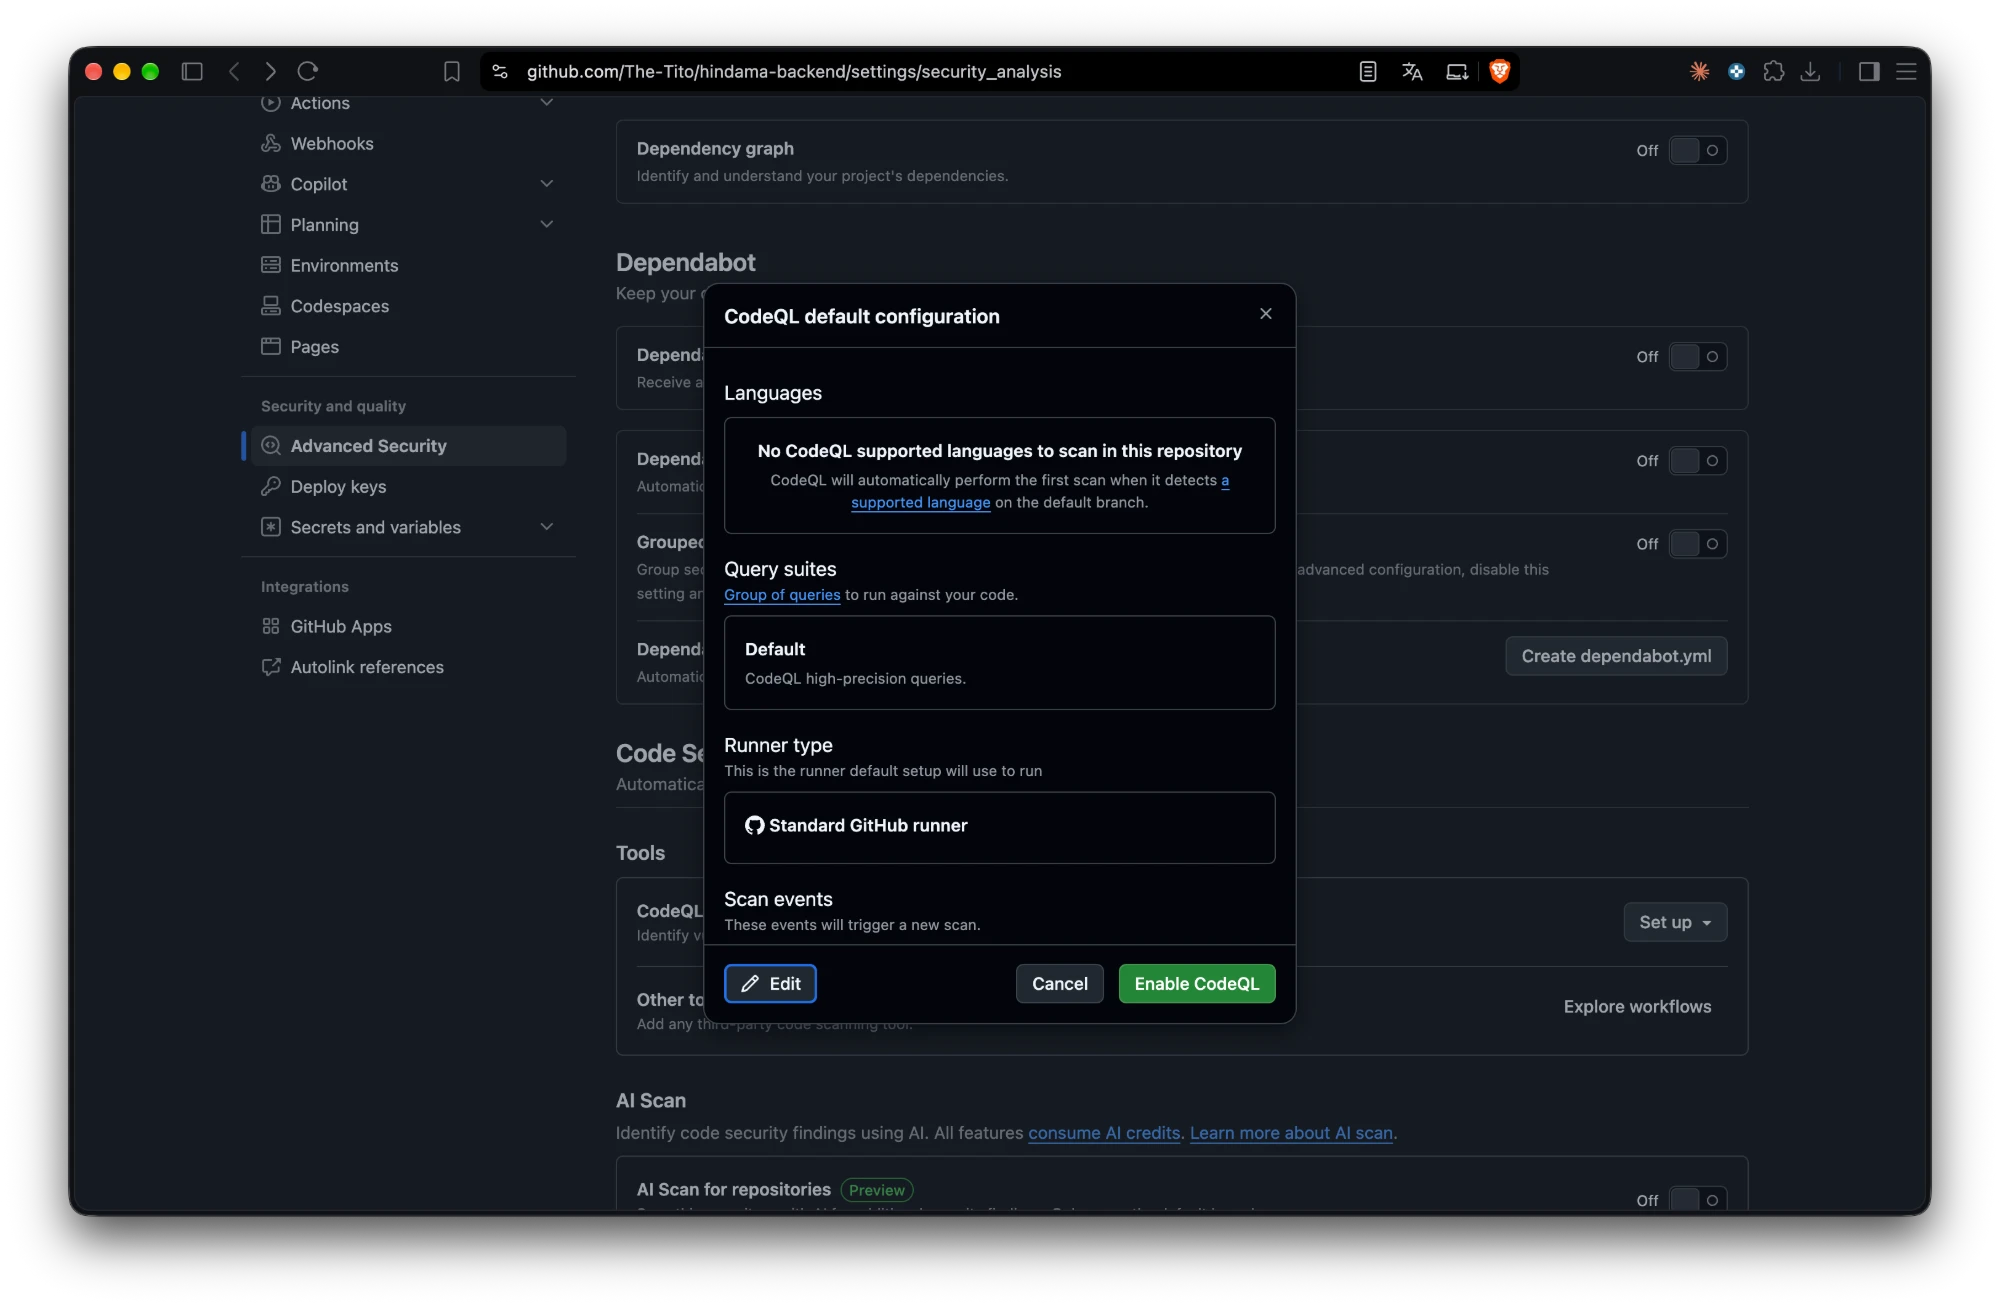
\includegraphics[width=0.9\linewidth]{img/captura-1a-sin-lenguajes.png}
  \caption{Default setup sin lenguajes compatibles en la rama predeterminada \texttt{main}.}
  \label{fig:sinlenguajes}
\end{figure}

\textbf{Causa.} El Default setup solo analiza la \textbf{rama predeterminada}. El proyecto sigue \emph{git flow} y su rama \cod{main} todavía no tiene ninguna entrega: contiene solo un README y \cod{.gitignore}, mientras que el código vive en \cod{develop}. Se cambió la rama predeterminada a \cod{develop}, pero GitHub siguió detectando únicamente GitHub Actions (figura~\ref{fig:soloactions}), porque su detector de lenguajes (Linguist) no se recalcula de inmediato tras el cambio.

\begin{figure}[H]\centering
  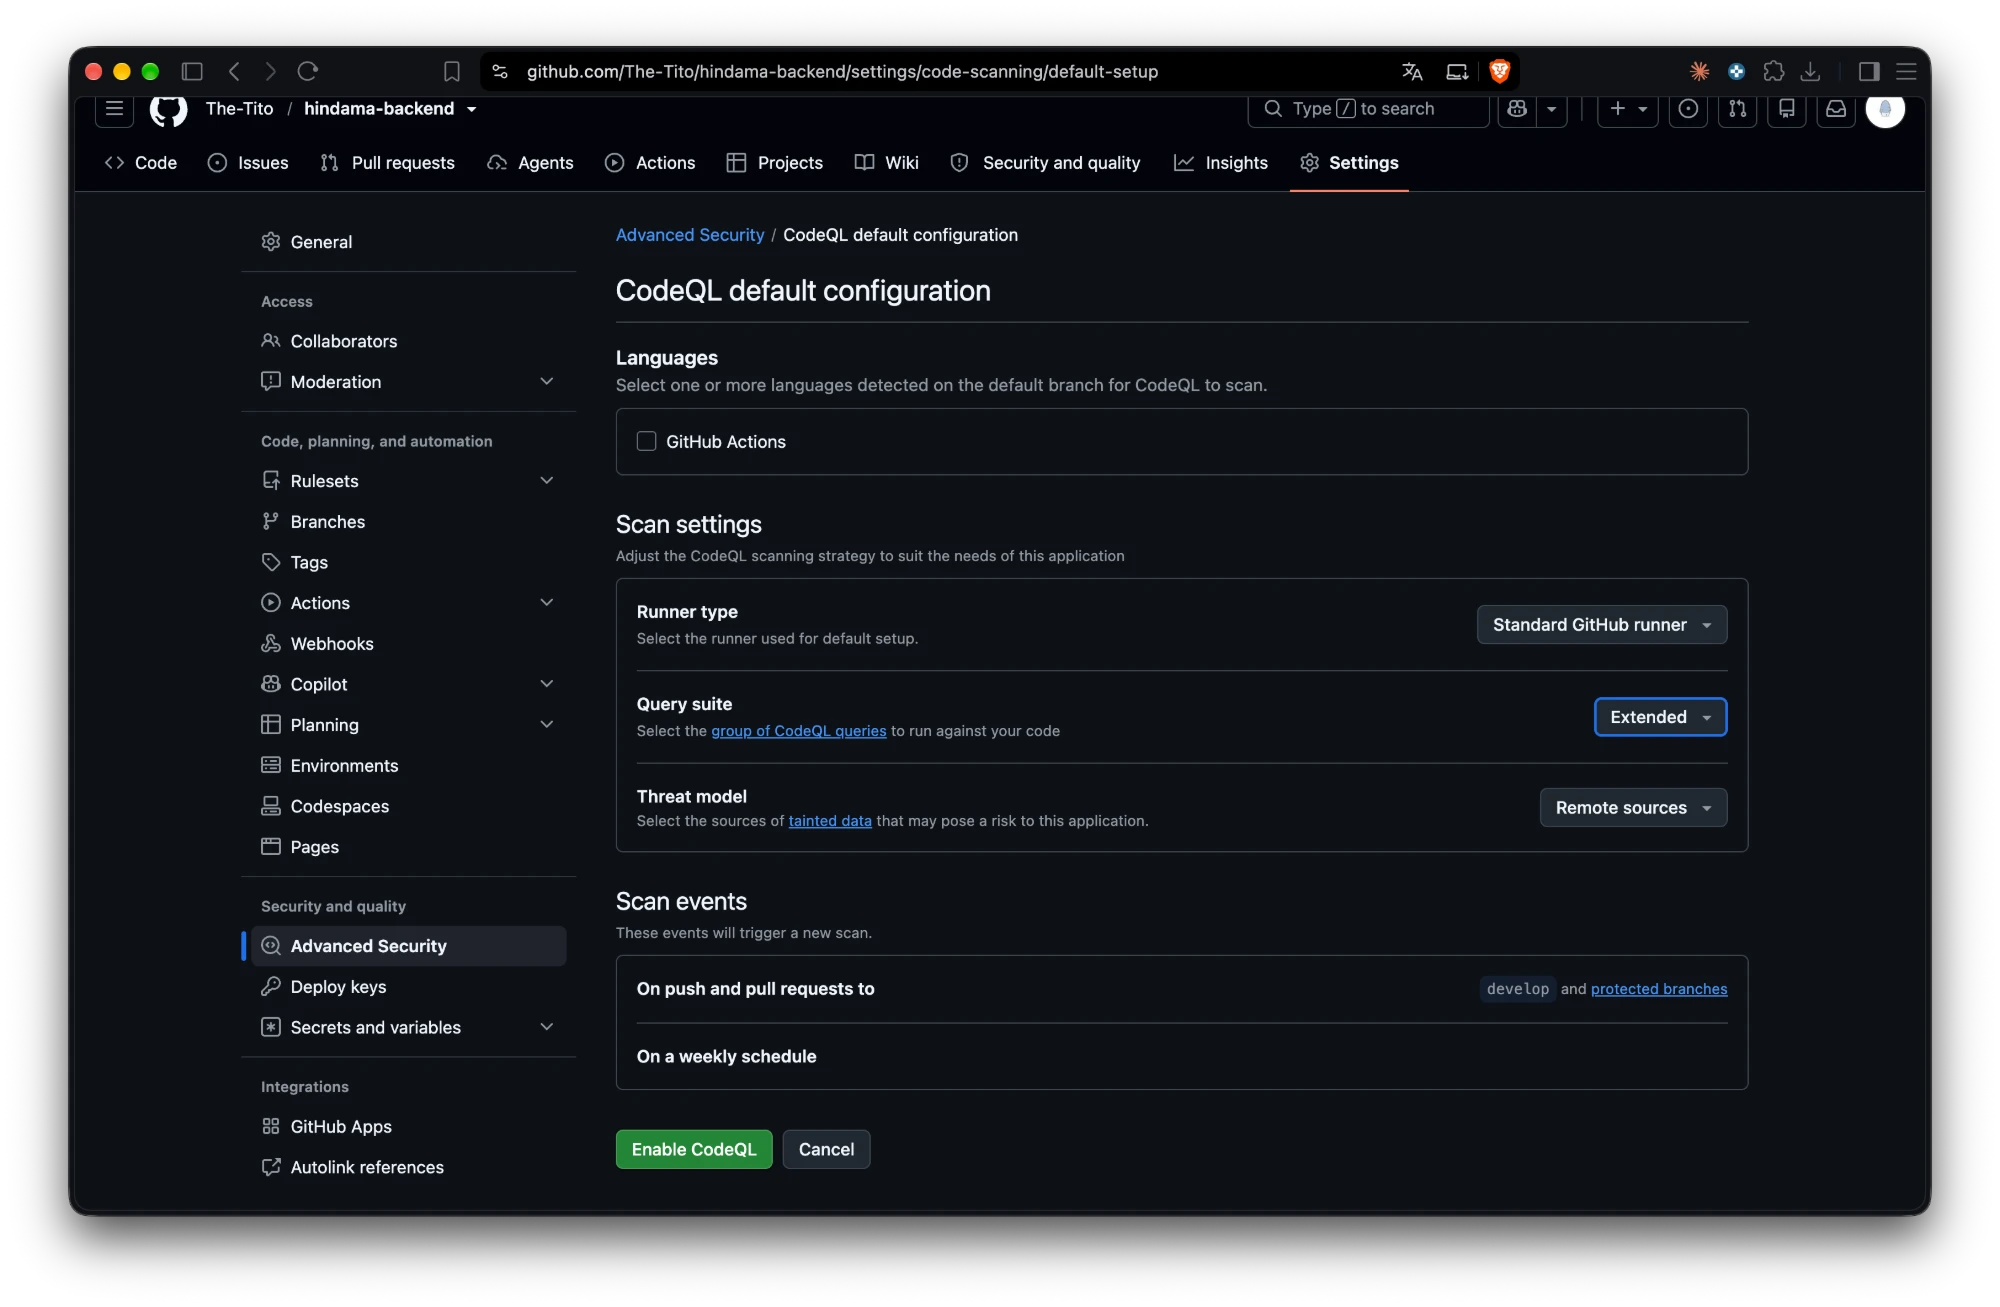
\includegraphics[width=0.9\linewidth]{img/captura-1b-solo-actions.png}
  \caption{Con \texttt{develop} como rama predeterminada, el Default setup aún solo ofrece GitHub Actions.}
  \label{fig:soloactions}
\end{figure}

\subsection{Decisión: Advanced setup con un workflow propio}

Se optó por el \textbf{Advanced setup}: un workflow propio que declara el lenguaje de forma explícita y no depende de la detección automática. Además, es el único modo que permite ejecutar consultas propias. El Default setup se dejó desactivado, porque ambos modos no pueden convivir. La rama predeterminada se mantuvo en \cod{develop}, que es donde se integra el trabajo.

\par\noindent\begin{minipage}{\linewidth}
\begin{lstlisting}[language=yaml,caption={Configuración \texttt{.github/codeql/codeql-config.yml}.}]
name: "Hindama CodeQL config"
queries:
  - uses: security-extended   # consultas estándar de seguridad
  - uses: ./codeql/queries    # nuestra consulta propia
paths-ignore:
  - tests
\end{lstlisting}
\end{minipage}\par

\par\noindent\begin{minipage}{\linewidth}
\begin{lstlisting}[language=yaml,caption={Workflow \texttt{.github/workflows/codeql.yml} (SHA abreviados).}]
name: CodeQL
on:
  push:
    branches: [main, develop]
  pull_request:
    branches: [main, develop]
  workflow_dispatch:
permissions:
  contents: read
  security-events: write
  actions: read
jobs:
  analyze:
    name: Analizar Python
    runs-on: ubuntu-latest
    timeout-minutes: 20
    steps:
      - uses: actions/checkout@3d3c42e5...            # v7.0.1
      - uses: github/codeql-action/init@33d7b85d...   # v4.39.3
        with:
          languages: python
          build-mode: none
          config-file: ./.github/codeql/codeql-config.yml
      - uses: github/codeql-action/analyze@33d7b85d... # v4.39.3
        with:
          category: "/language:python"
\end{lstlisting}
\end{minipage}\par

Las acciones se fijaron por SHA de commit, igual que en la CI existente del proyecto: si alguien moviera la etiqueta \cod{v4} a otro código, el workflow no cambiaría. Para que cada fase dejara evidencia separada, el trabajo se dividió en cuatro commits (tabla~\ref{tab:commits}).

\begin{table}[H]\centering
\caption{Commits de la práctica en la rama \texttt{practica/codeql}.}
\label{tab:commits}
\begin{tabularx}{\linewidth}{@{}p{1.7cm}Lp{4.2cm}@{}}
\toprule
\textbf{Commit} & \textbf{Contenido} & \textbf{Fase} \\ \midrule
\cod{2cb6330} & Workflow y configuración solo con \cod{security-extended} & Línea base \\
\cod{cb706b0} & Consulta propia y archivo demo con las 4 variantes & Detección de variantes \\
\cod{50e0669} & Corrección con parámetros enlazados & Eliminación y verificación \\
\cod{f27348f} & Retiro del archivo demo & Integración a \cod{develop} \\ \bottomrule
\end{tabularx}
\end{table}

% ======================= 4 =======================
\section{Análisis inicial (línea base)}

El primer análisis aplicó las \textbf{50 reglas} de \cod{security-extended} sobre los \textbf{97 archivos} del backend. El run terminó en verde en 50 segundos (figura~\ref{fig:runbase}).

\begin{figure}[H]\centering
  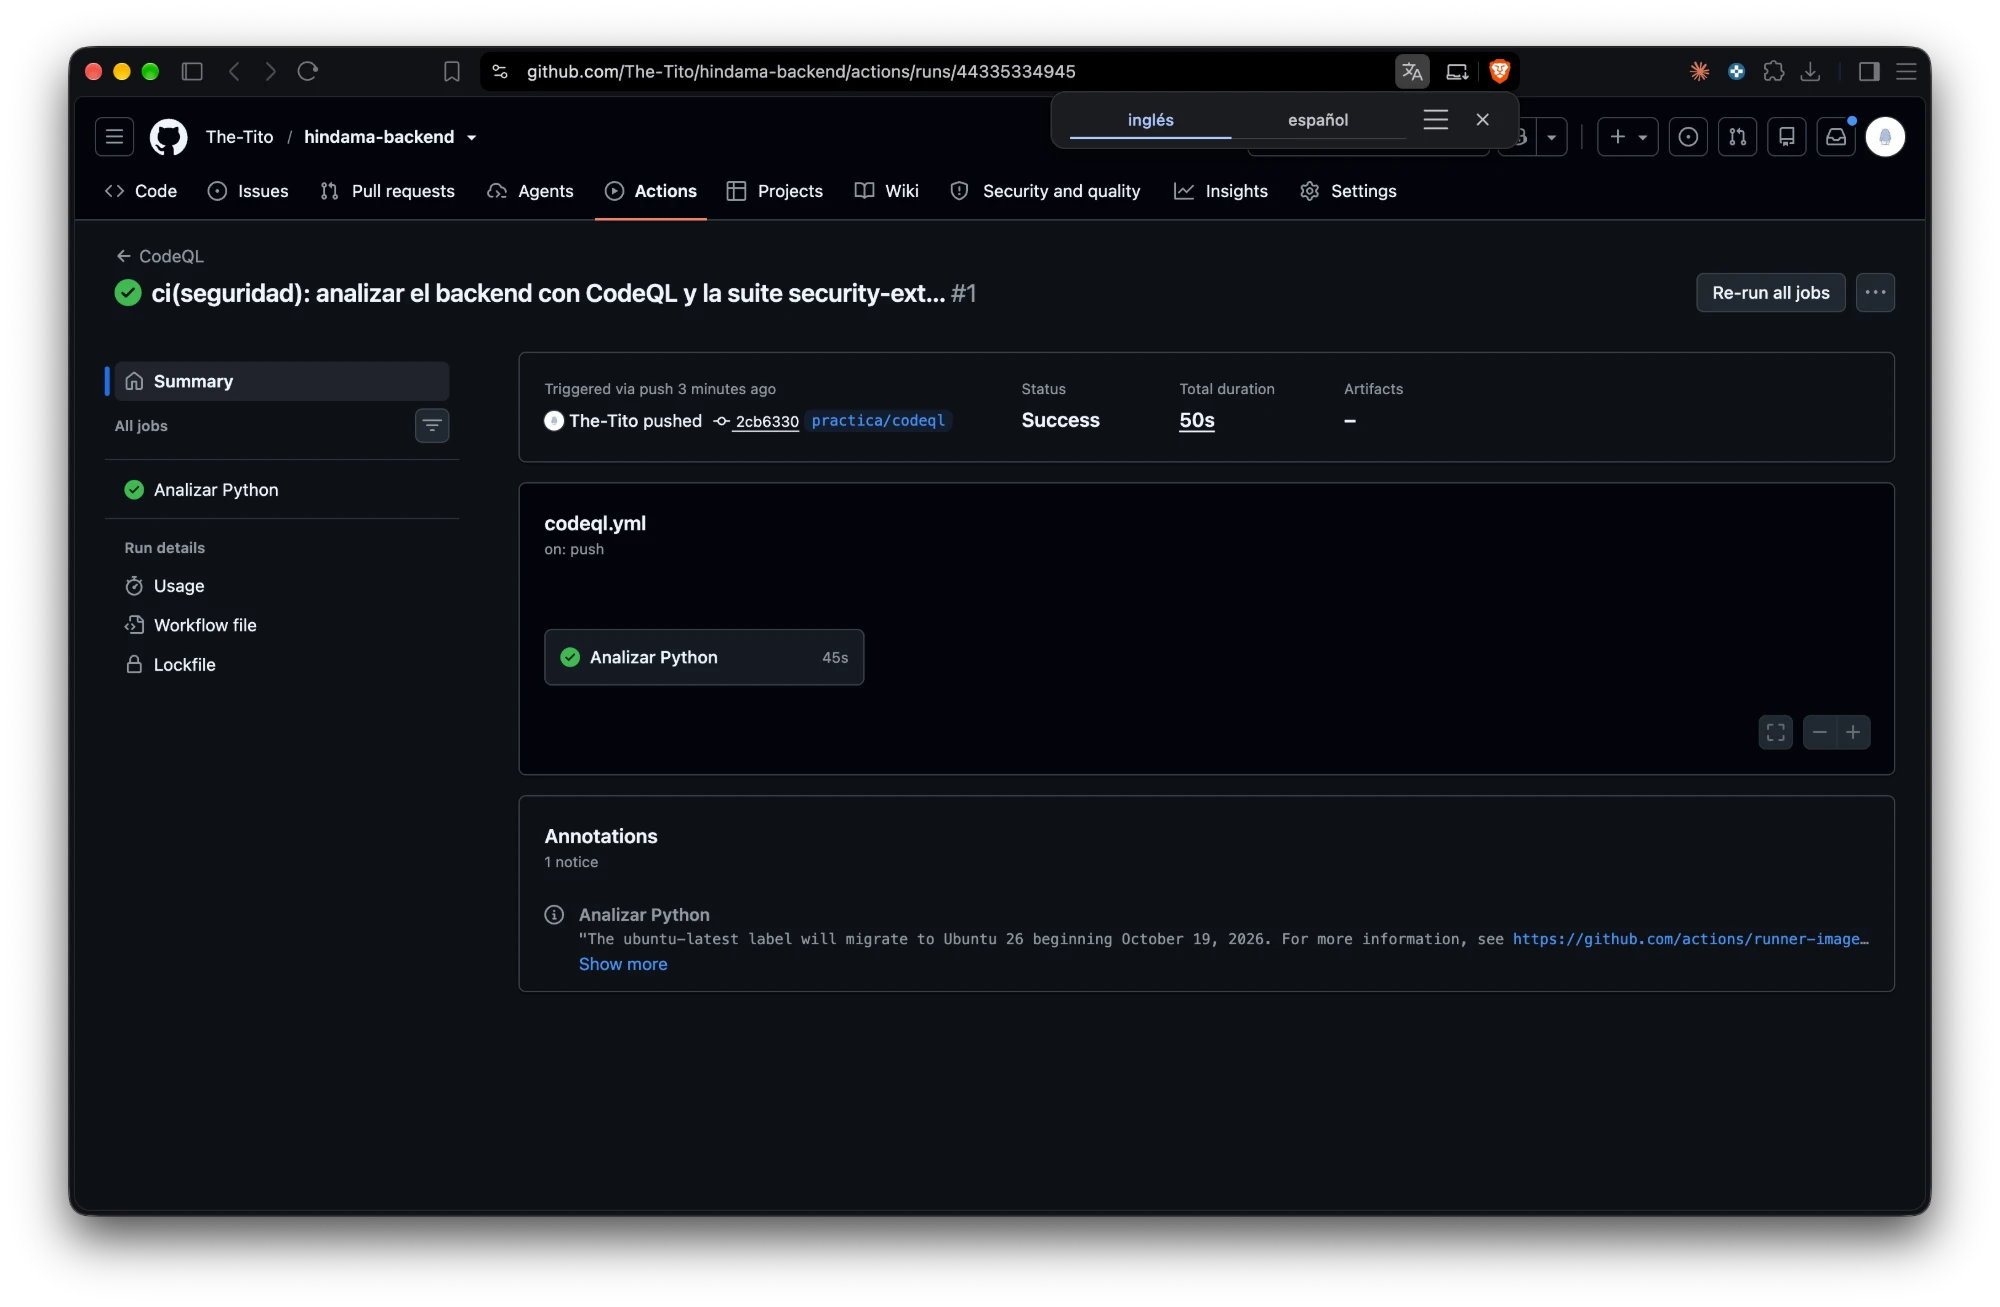
\includegraphics[width=0.9\linewidth]{img/captura-2-run-linea-base.png}
  \caption{Run de la línea base (commit \texttt{2cb6330}) terminado con éxito.}
  \label{fig:runbase}
\end{figure}

\textbf{Resultado: 0 alertas.} Code Scanning no reportó ningún hallazgo abierto ni cerrado en la rama (figura~\ref{fig:ceroalertas}).

\begin{figure}[H]\centering
  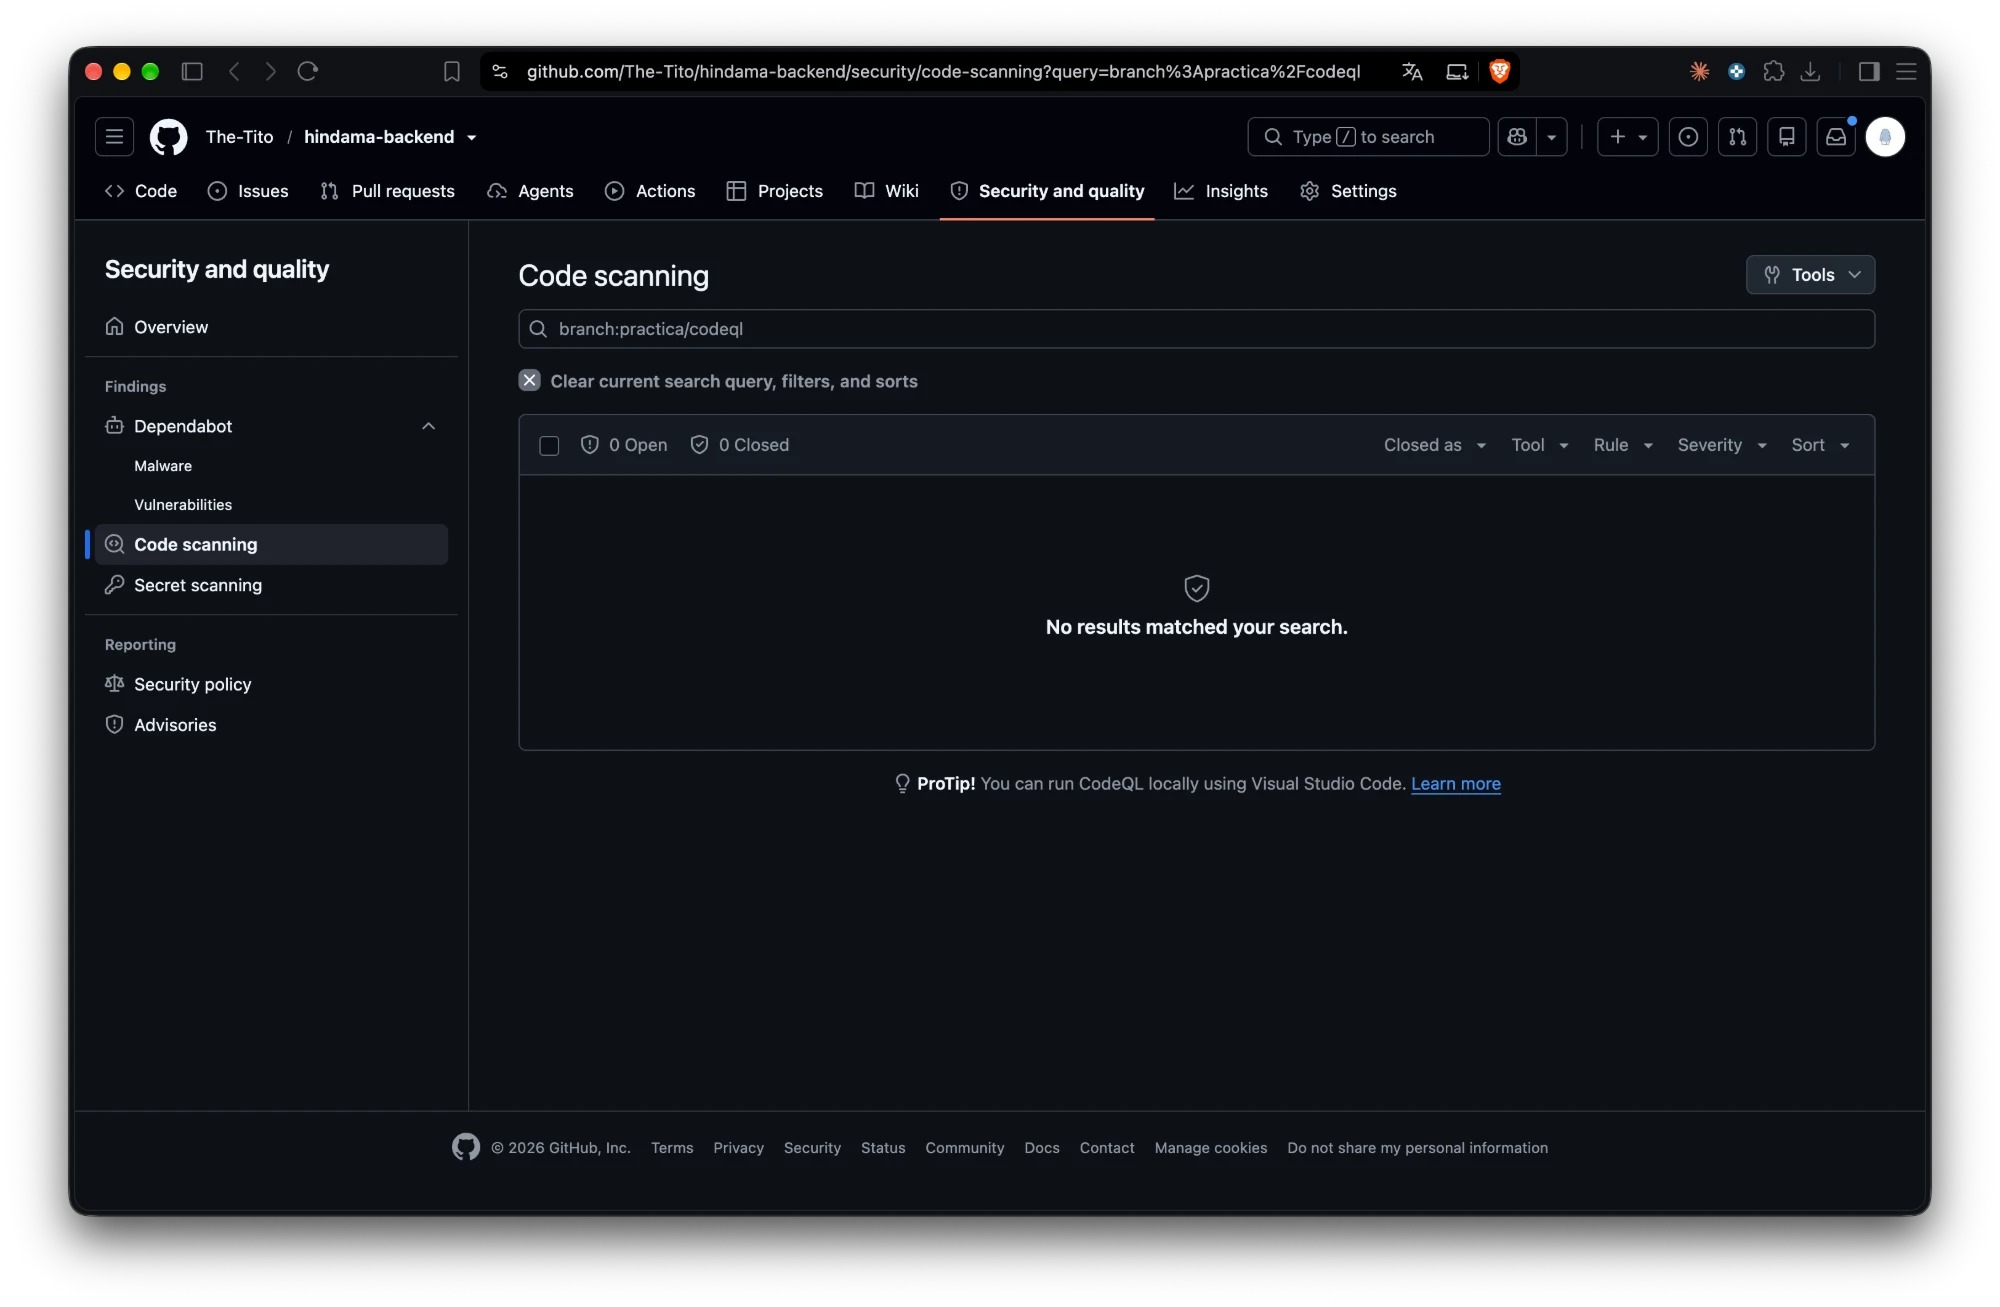
\includegraphics[width=0.9\linewidth]{img/captura-3-cero-alertas.png}
  \caption{Code Scanning filtrado por la rama \texttt{practica/codeql}: 0 alertas en la línea base.}
  \label{fig:ceroalertas}
\end{figure}

\begin{table}[H]\centering
\caption{Datos del análisis inicial.}
\begin{tabularx}{\linewidth}{@{}p{4.2cm}L@{}}
\toprule
\textbf{Dato} & \textbf{Valor} \\ \midrule
ID del análisis & 2197004800 \\
Versión de CodeQL & 2.27.4 \\
Reglas aplicadas & 50 \\
Resultados & 0 \\
Evidencia & \cod{linea-base.sarif}, \cod{alertas-linea-base.json}, \cod{archivos-analizados.txt} \\ \bottomrule
\end{tabularx}
\end{table}

\textbf{Interpretación.} Un resultado limpio es coherente con el diseño del proyecto: las consultas a la base de datos usan el ORM o SQL literal con parámetros enlazados; las peticiones salientes pasan por una guardia SSRF obligatoria; y la CI ya ejecuta las reglas de Bandit de \emph{ruff}, \emph{pip-audit} y \emph{Trivy}. Aun así, un cero de las consultas estándar no garantiza la ausencia de fallas: solo cubren los patrones que GitHub generalizó. Por eso el siguiente paso fue escribir una consulta específica para el proyecto.

% ======================= 5 =======================
\section{Consulta personalizada}

\subsection{La vulnerabilidad elegida}

Se eligió \textbf{inyección SQL (CWE-89) en \cod{sqlalchemy.text()}}, la función con la que SQLAlchemy, el ORM del proyecto, ejecuta SQL escrito a mano. La consulta estándar \cod{py/sql-injection} es de flujo de datos (\emph{taint tracking}): solo avisa cuando puede seguir el dato desde una fuente remota, como un parámetro HTTP, hasta la consulta. Si el valor viene de la base de datos, de un archivo, de una cola o de una función que el motor no modela, no hay alerta.

La consulta propia invierte el enfoque: marca \textbf{cualquier} SQL construido con operaciones de texto dentro de \cod{text()}, venga de donde venga el dato. Detecta las cuatro formas de armar texto en Python (tabla~\ref{tab:variantes}).

\begin{table}[H]\centering
\caption{Variantes que detecta la consulta.}
\label{tab:variantes}
\begin{tabularx}{\linewidth}{@{}p{3cm}Lp{4.6cm}@{}}
\toprule
\textbf{Variante} & \textbf{Ejemplo} & \textbf{Nodo QL que la detecta} \\ \midrule
f-string & \cod{text(f"... \{x\}")} & \cod{Fstring} \\
Concatenación & \cod{text("..." + x)} & \cod{BinaryExpr} con \cod{Add} \\
Operador \% & \cod{text("... \%s" \% x)} & \cod{BinaryExpr} con \cod{Mod} \\
\cod{.format()} & \cod{text("... \{\}".format(x))} & \cod{Call} al atributo \cod{format} \\ \bottomrule
\end{tabularx}
\end{table}

\subsection{Código de la consulta}

La consulta vive en \cod{codeql/queries/SqlTextDinamico.ql}. El archivo \cod{qlpack.yml} la declara como el paquete \cod{hindama/python-queries}, que depende de la biblioteca estándar de Python de CodeQL:

\par\noindent\begin{minipage}{\linewidth}
\begin{lstlisting}[language=yaml,caption={\texttt{codeql/queries/qlpack.yml}.}]
name: hindama/python-queries
version: 0.0.1
dependencies:
  codeql/python-all: "*"
\end{lstlisting}
\end{minipage}\par

\lstinputlisting[language=QL,caption={\texttt{codeql/queries/SqlTextDinamico.ql}.},label={lst:ql}]{../../codeql/queries/SqlTextDinamico.ql}

\begin{figure}[H]\centering
  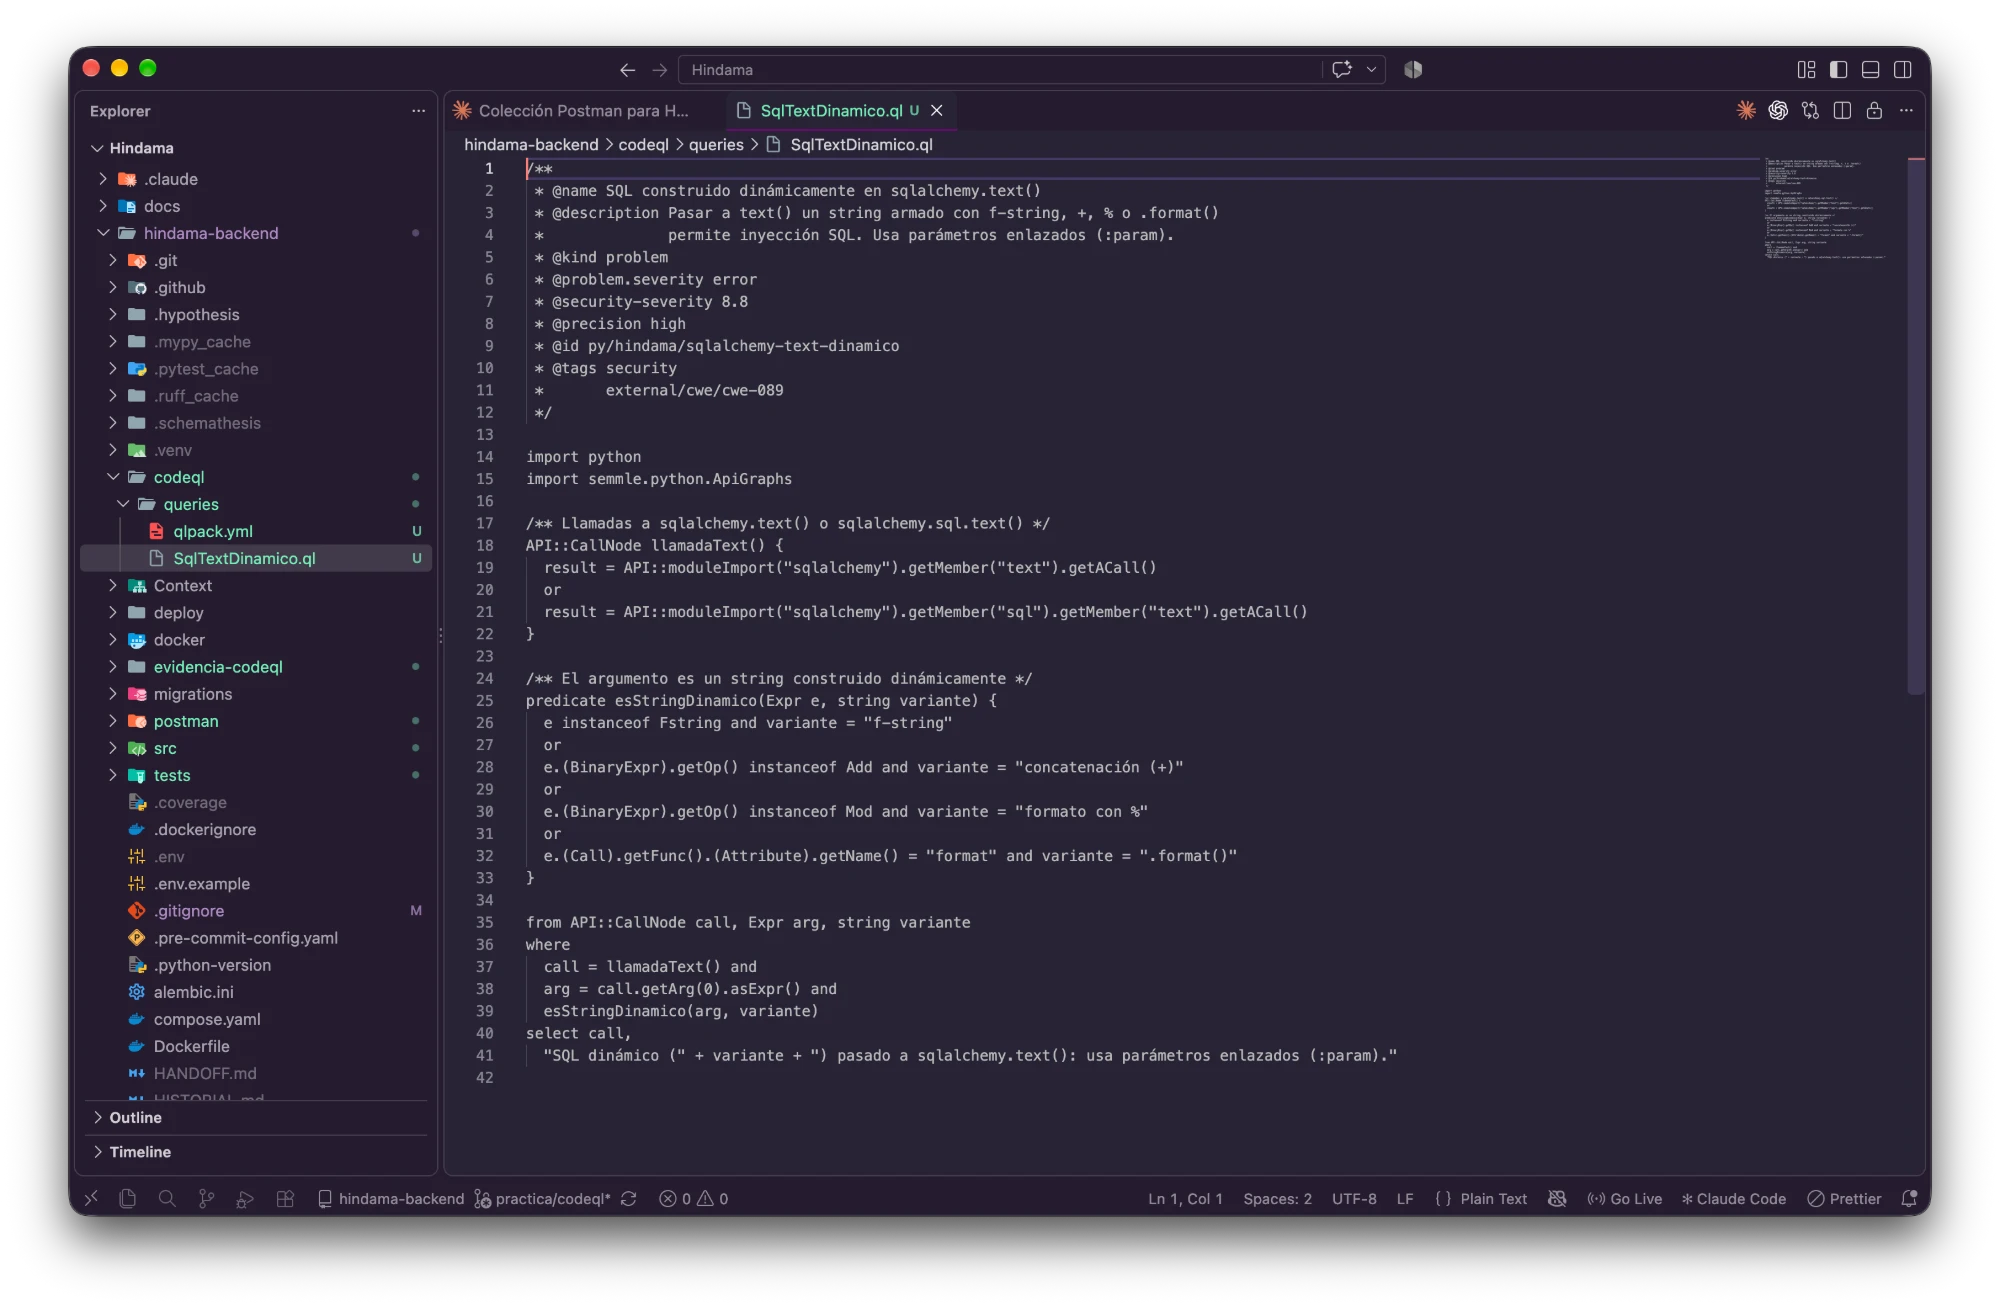
\includegraphics[width=0.9\linewidth]{img/captura-4-consulta-ql.png}
  \caption{La consulta \texttt{SqlTextDinamico.ql} en el editor.}
\end{figure}

\subsection{Cómo funciona}

\begin{itemize}
  \item \textbf{Metadatos.} \cod{@kind problem} produce una alerta por resultado; \cod{@security-severity 8.8} hace que GitHub la clasifique como \emph{High}; \cod{@id} y la etiqueta \cod{external/cwe/cwe-089} la identifican en Code Scanning.
  \item \textbf{\cod{llamadaText()}.} Usa \emph{API Graphs}, que siguen los \emph{imports}: encuentra \cod{sqlalchemy.text} y \cod{sqlalchemy.sql.text} aunque se importen con otro nombre (\cod{from sqlalchemy import text as t}).
  \item \textbf{\cod{esStringDinamico()}.} Revisa el árbol sintáctico del primer argumento y devuelve qué variante encontró, para que el mensaje de la alerta la nombre.
  \item \textbf{\cod{select}.} Reporta la llamada a \cod{text()} con un mensaje que indica la corrección: usar parámetros enlazados (\cod{:param}).
\end{itemize}

% ======================= 6 =======================
\section{Detección de las variantes}

El código real del backend no tiene ninguna de las cuatro variantes. Para demostrar que la consulta funciona, se creó un caso controlado, \cod{src/hindama/demo\_codeql.py}, con una función por variante:

\begin{lstlisting}[language=Python,caption={Caso vulnerable controlado (commit \texttt{cb706b0}).}]
"""Archivo de demostración para la práctica de CodeQL. NO usar en producción."""

from sqlalchemy import text
from sqlalchemy.ext.asyncio import AsyncSession


async def variante_fstring(session: AsyncSession, nombre: str):
    return await session.execute(text(f"SELECT * FROM usuarios WHERE nombre = '{nombre}'"))


async def variante_concatenacion(session: AsyncSession, nombre: str):
    return await session.execute(text("SELECT * FROM usuarios WHERE nombre = '" + nombre + "'"))


async def variante_porcentaje(session: AsyncSession, nombre: str):
    return await session.execute(text("SELECT * FROM usuarios WHERE nombre = '%s'" % nombre))


async def variante_format(session: AsyncSession, nombre: str):
    return await session.execute(text("SELECT * FROM usuarios WHERE nombre = '{}'".format(nombre)))
\end{lstlisting}

Con la consulta propia agregada a la configuración, el análisis aplicó \textbf{51 reglas} (las 50 estándar y la nueva) y terminó en verde (figura~\ref{fig:runpropia}).

\begin{figure}[H]\centering
  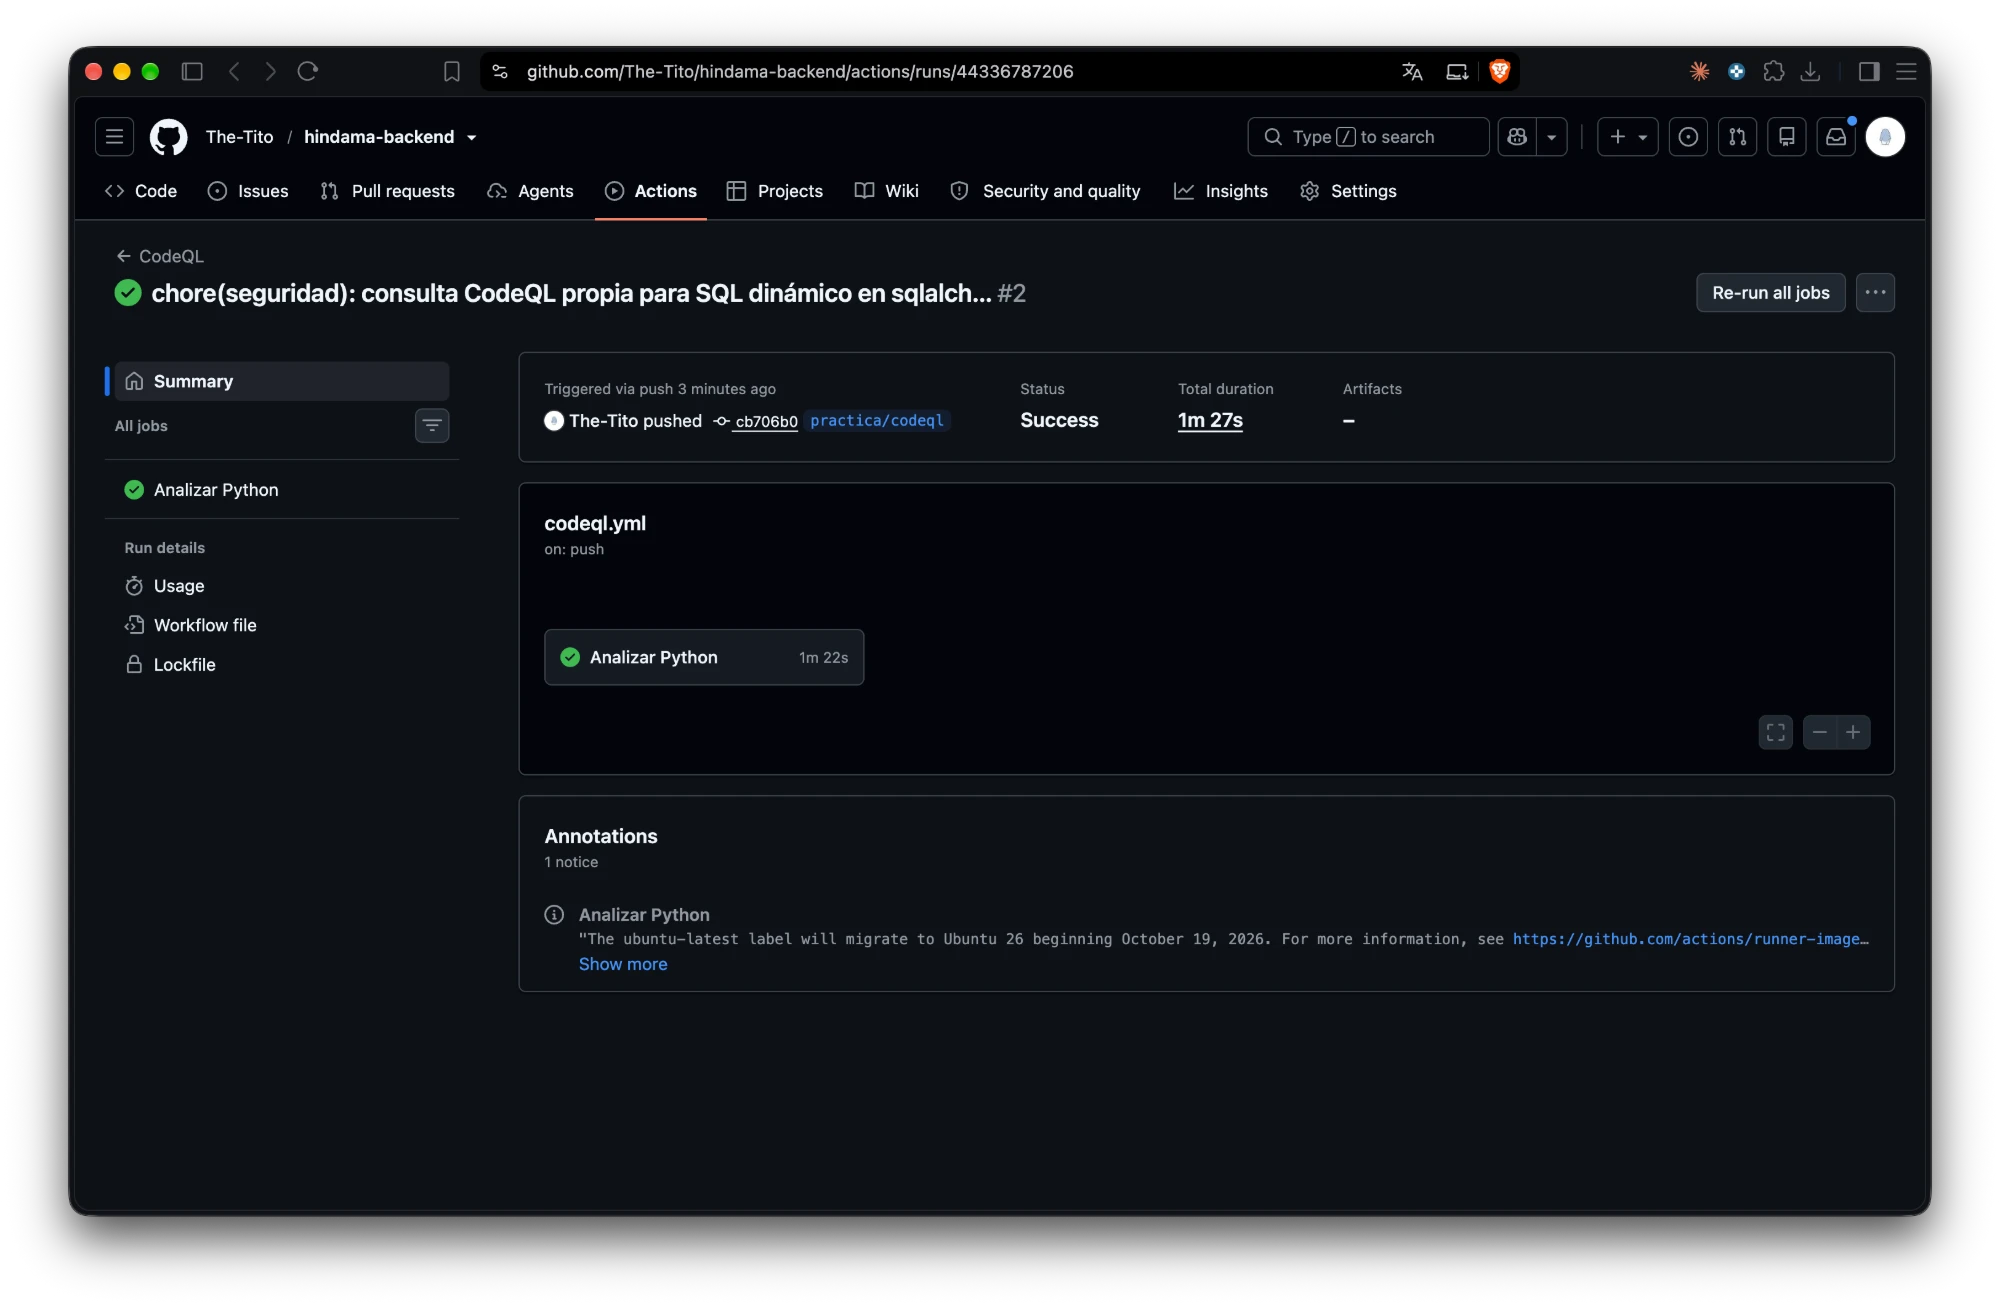
\includegraphics[width=0.9\linewidth]{img/captura-5-run-consulta-propia.png}
  \caption{Run con la consulta propia (commit \texttt{cb706b0}) terminado con éxito.}
  \label{fig:runpropia}
\end{figure}

La consulta encontró \textbf{exactamente 4 alertas, una por variante}, todas de severidad \emph{High} (figura~\ref{fig:cuatro} y tabla~\ref{tab:alertas}).

\begin{figure}[H]\centering
  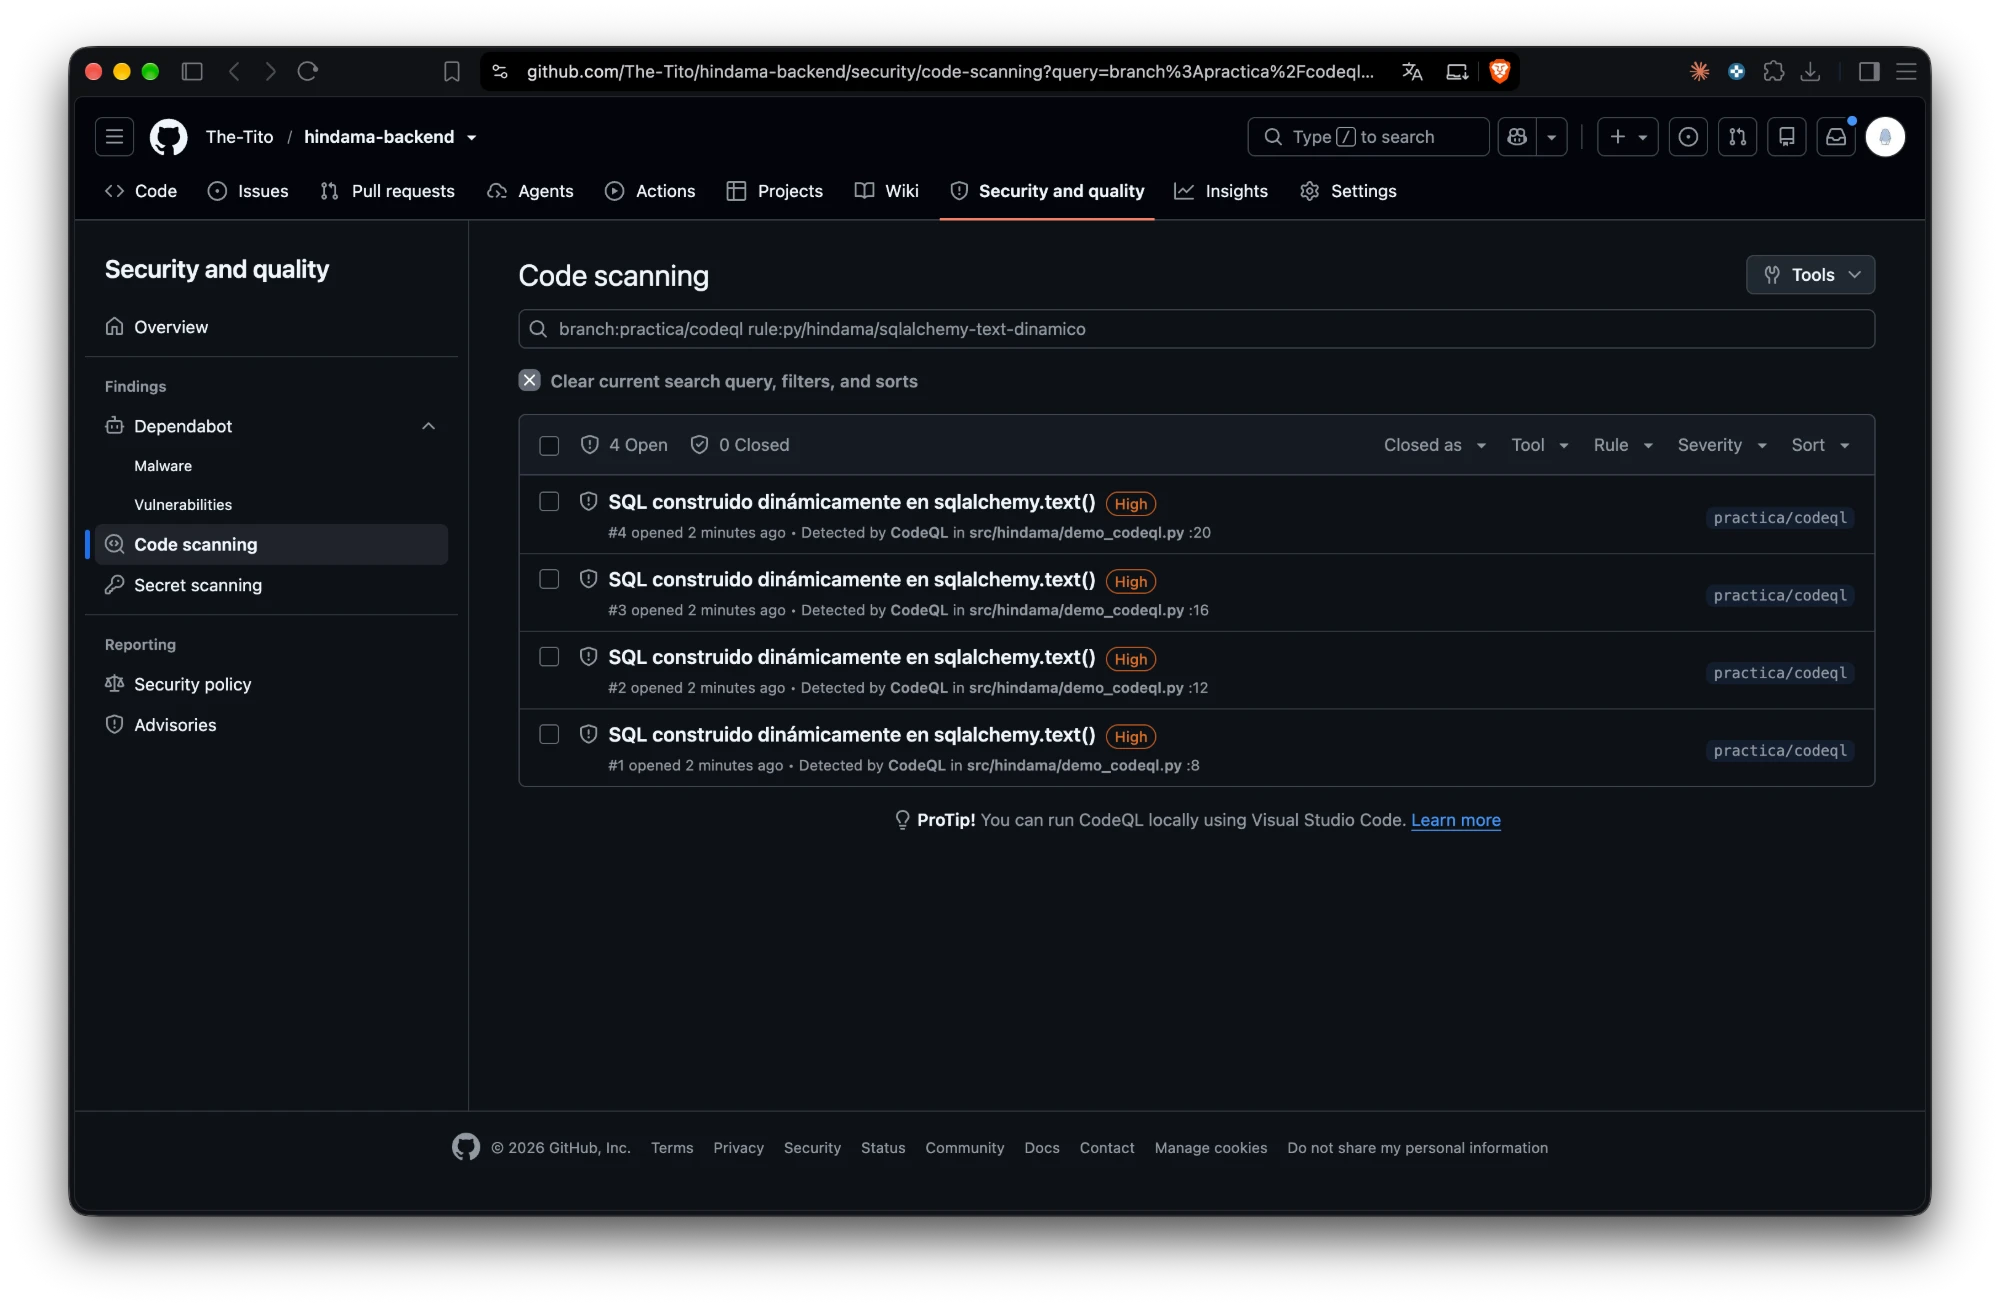
\includegraphics[width=0.9\linewidth]{img/captura-6-cuatro-alertas.png}
  \caption{Las 4 alertas de \texttt{py/hindama/sqlalchemy-text-dinamico}, abiertas en la rama.}
  \label{fig:cuatro}
\end{figure}

\begin{table}[H]\centering
\caption{Alertas generadas por la consulta propia.}
\label{tab:alertas}
\begin{tabularx}{\linewidth}{@{}p{0.6cm}p{3.3cm}Lp{3.4cm}@{}}
\toprule
\textbf{\#} & \textbf{Variante} & \textbf{Mensaje} & \textbf{Ubicación} \\ \midrule
1 & f-string & SQL dinámico (f-string) pasado a \cod{sqlalchemy.text()} & \cod{demo\_codeql.py:8} \\
2 & Concatenación (+) & SQL dinámico (concatenación (+)) pasado a \cod{sqlalchemy.text()} & \cod{demo\_codeql.py:12} \\
3 & Formato con \% & SQL dinámico (formato con \%) pasado a \cod{sqlalchemy.text()} & \cod{demo\_codeql.py:16} \\
4 & \cod{.format()} & SQL dinámico (.format()) pasado a \cod{sqlalchemy.text()} & \cod{demo\_codeql.py:20} \\ \bottomrule
\end{tabularx}
\end{table}

\subsection{Comparación con otras herramientas}

\begin{table}[H]\centering
\caption{Variantes detectadas por cada herramienta sobre el mismo archivo.}
\begin{tabularx}{\linewidth}{@{}p{4.6cm}p{2.3cm}L@{}}
\toprule
\textbf{Herramienta} & \textbf{Detectadas} & \textbf{Observación} \\ \midrule
CodeQL \cod{security-extended} (\cod{py/sql-injection}) & 0 de 4 & El dato no proviene de una fuente remota modelada, así que el análisis de flujo no lo considera contaminado. \\
Consulta propia & \textbf{4 de 4} & Detecta la forma del SQL, sin importar el origen del dato. \\
\emph{ruff}, regla S608 (Bandit) & 4 de 4 & Ya corre en la CI del proyecto; trabaja por patrones sobre cadenas con palabras de SQL. \\ \bottomrule
\end{tabularx}
\end{table}

\textbf{Falsos positivos: ninguno.} El backend tiene unas veinte llamadas legítimas a \cod{text()} (valores por omisión de columnas, índices parciales y la configuración de Row-Level Security con parámetros enlazados), y la consulta no marcó ninguna.

% ======================= 7 =======================
\section{Corrección}

Las cuatro funciones vulnerables se reemplazaron por una sola consulta con un \textbf{parámetro enlazado} (\cod{:nombre}):

\par\noindent\begin{minipage}{\linewidth}
\begin{lstlisting}[language=Python,caption={Versión corregida (commit \texttt{50e0669}).}]
"""Archivo de demostración para la práctica de CodeQL (versión corregida)."""

from sqlalchemy import text
from sqlalchemy.ext.asyncio import AsyncSession

CONSULTA = text("SELECT * FROM usuarios WHERE nombre = :nombre")


async def buscar_usuario(session: AsyncSession, nombre: str):
    return await session.execute(CONSULTA, {"nombre": nombre})
\end{lstlisting}
\end{minipage}\par

\begin{figure}[H]\centering
  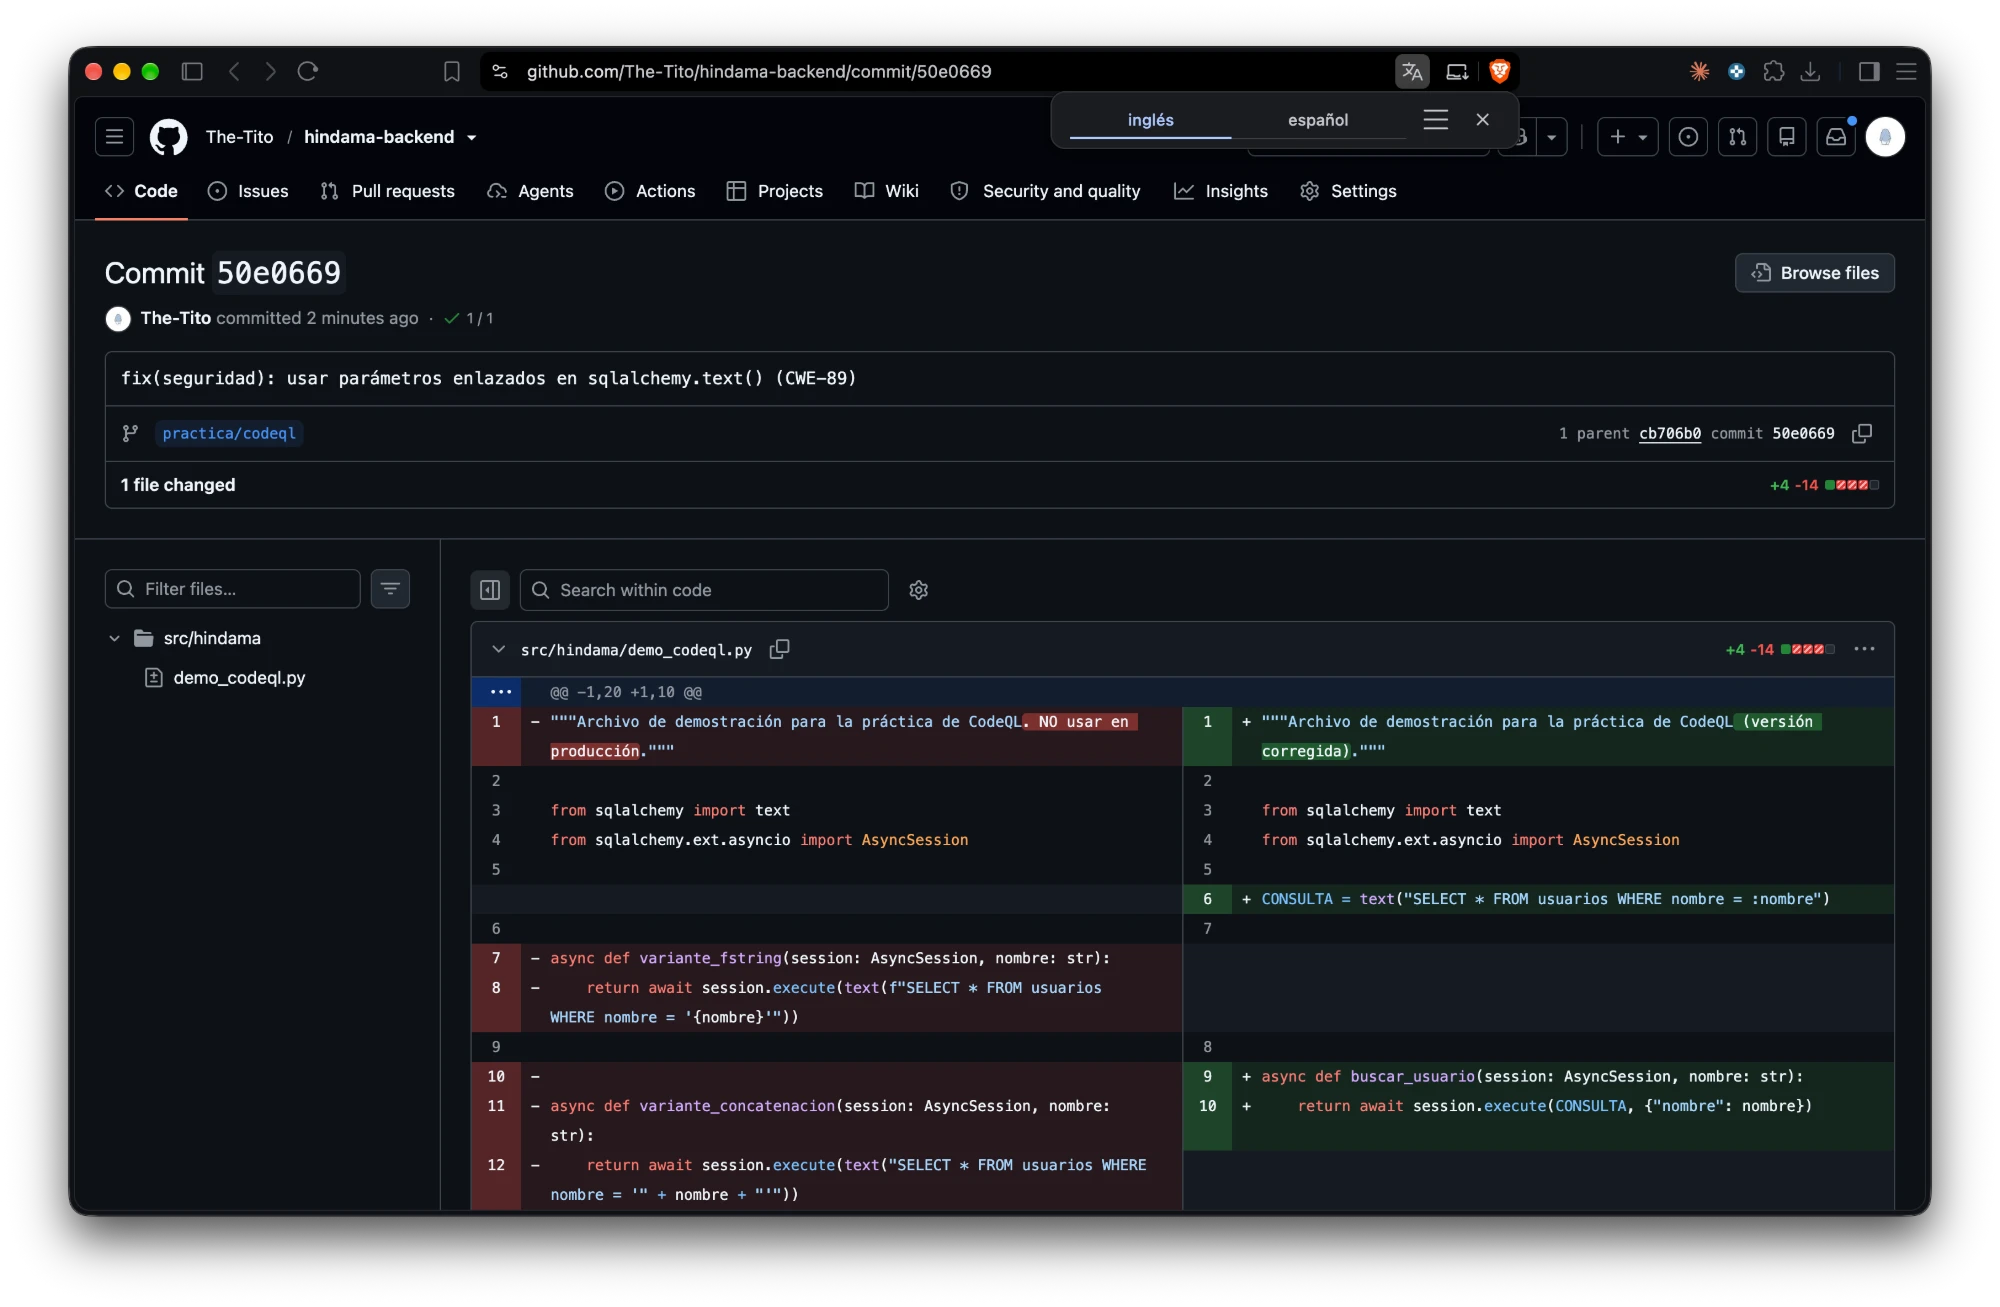
\includegraphics[width=0.9\linewidth]{img/captura-7-diff-correccion.png}
  \caption{Diff del commit \texttt{50e0669}: las cuatro variantes se sustituyen por una consulta parametrizada.}
\end{figure}

\textbf{Por qué elimina la vulnerabilidad.} Con un parámetro enlazado, el texto SQL y el dato viajan por separado: el controlador de PostgreSQL envía la sentencia con un marcador y el valor aparte, y la base de datos nunca interpreta el valor como código. Una entrada como \cod{' OR '1'='1} se compara literalmente como nombre y no altera la consulta. Además, la sentencia queda fija en una constante, de modo que no se puede construir con datos de la petición.

% ======================= 8 =======================
\section{Verificación}

Tras subir la corrección, CodeQL volvió a analizar la rama: \textbf{51 reglas y 0 resultados}. GitHub cerró automáticamente las cuatro alertas como \emph{Fixed} (figura~\ref{fig:fixed}).

\begin{figure}[H]\centering
  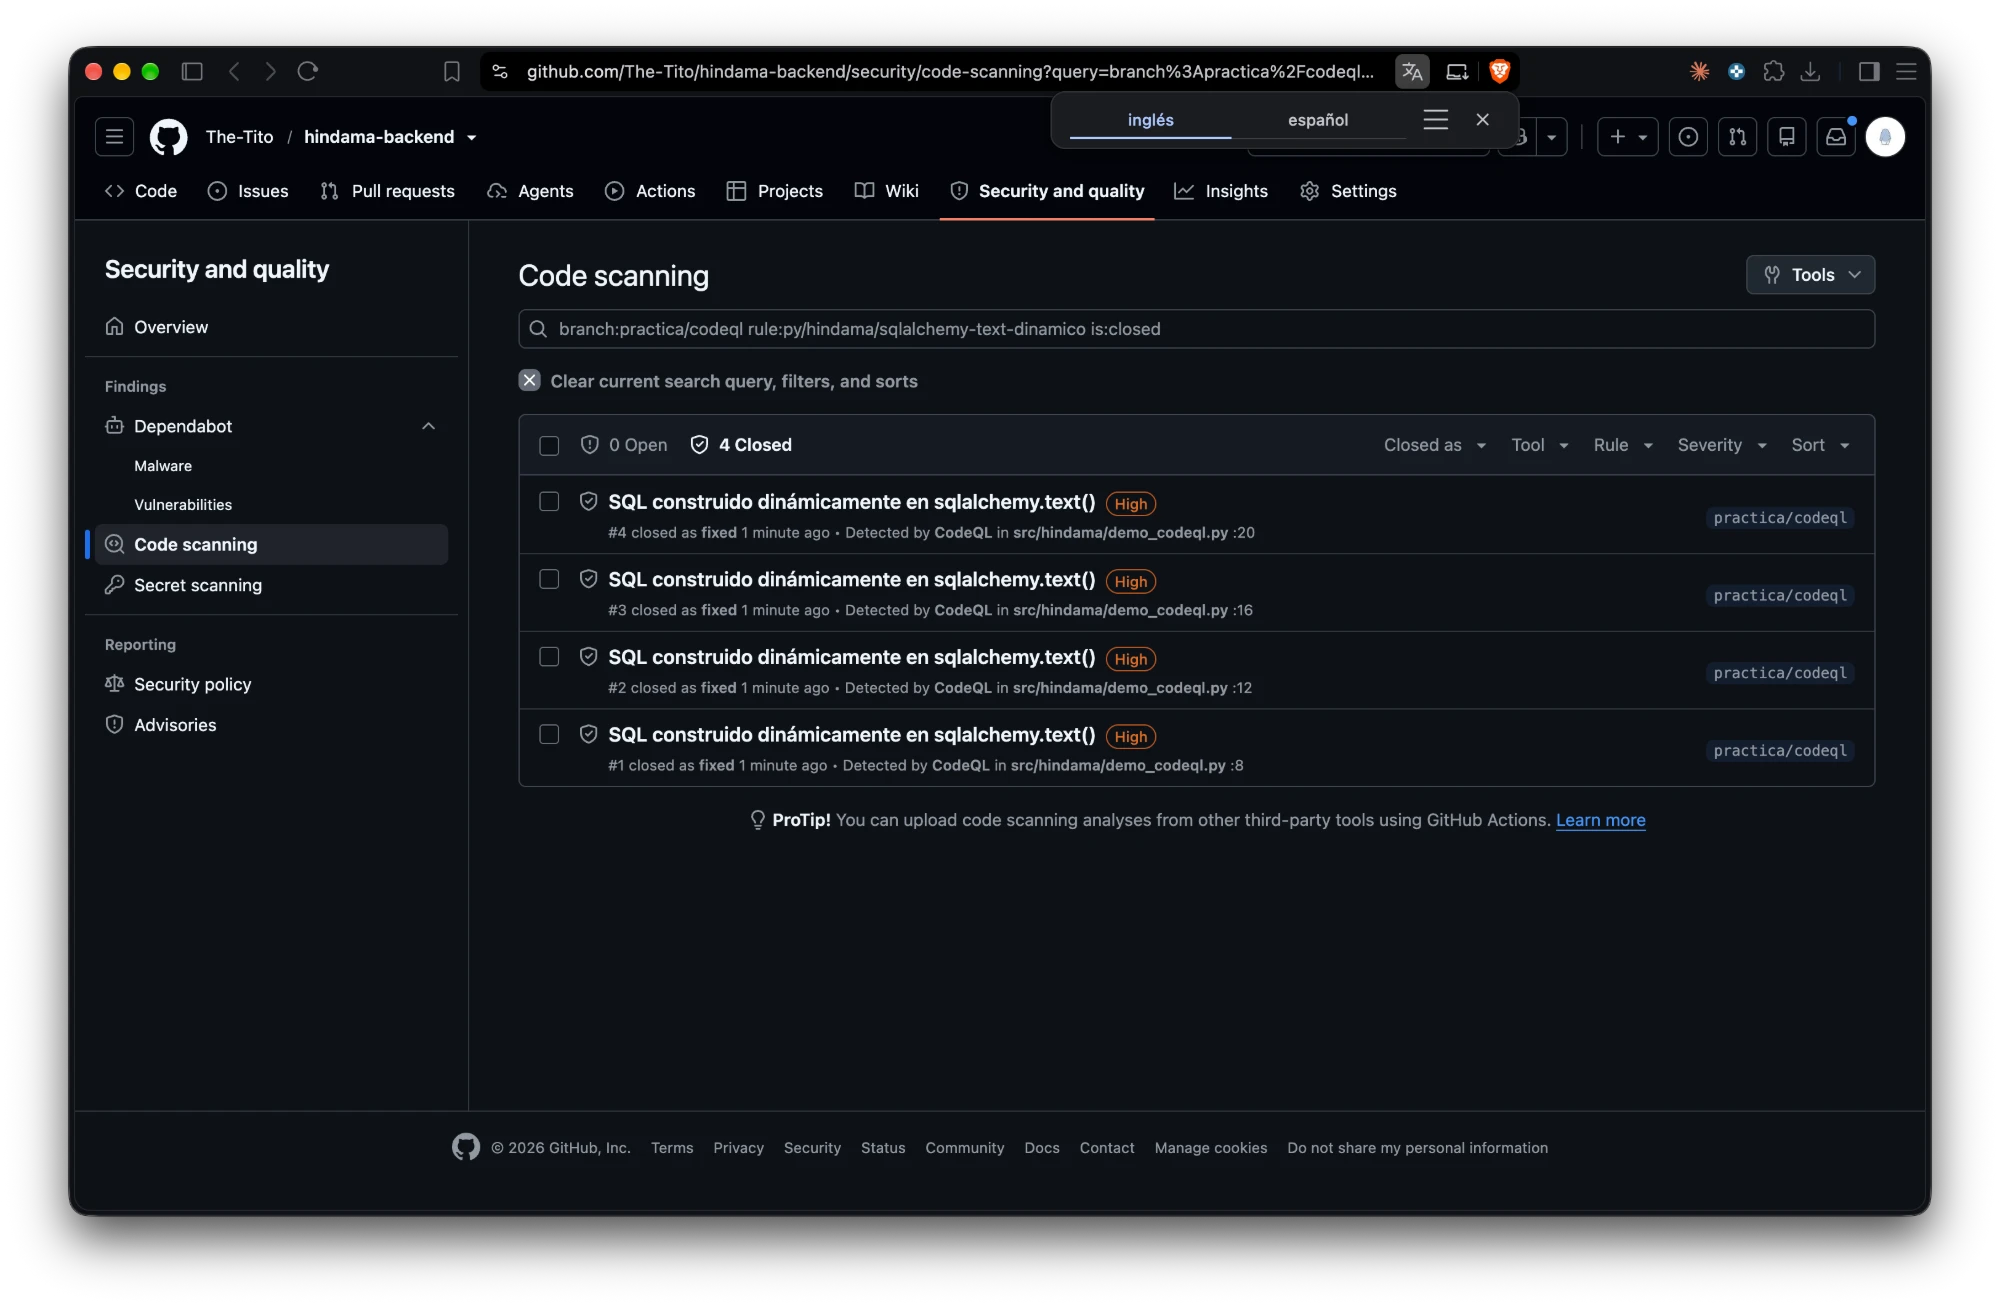
\includegraphics[width=0.9\linewidth]{img/captura-8-alertas-fixed.png}
  \caption{Las 4 alertas cerradas como \emph{fixed} tras la corrección.}
  \label{fig:fixed}
\end{figure}

\begin{table}[H]\centering
\caption{Estado final de las alertas.}
\begin{tabularx}{0.7\linewidth}{@{}p{2cm}p{2.2cm}L@{}}
\toprule
\textbf{Alerta} & \textbf{Estado} & \textbf{Cerrada el (UTC)} \\ \midrule
\#1 & fixed & 2026-11-18 15:39:50 \\
\#2 & fixed & 2026-11-18 15:39:50 \\
\#3 & fixed & 2026-11-18 15:39:50 \\
\#4 & fixed & 2026-11-18 15:39:50 \\ \bottomrule
\end{tabularx}
\end{table}

Después se retiró el archivo de demostración (commit \cod{f27348f}), de modo que a \cod{develop} solo llegan la consulta, su configuración y el workflow.

% ======================= 9 =======================
\section{Compartir la consulta}

La consulta se comparte de tres formas:

\begin{enumerate}
  \item \textbf{En el repositorio público.} Queda en \cod{codeql/queries/} y se integra a \cod{develop} mediante el \href{https://github.com/The-Tito/hindama-backend/pull/27}{pull request \#27}. En ese PR pasaron los seis controles: CodeQL, \emph{Analizar Python}, \emph{Lint y tipos}, \emph{Pruebas, migraciones y contrato}, \emph{Dependencias vulnerables} e \emph{Imagen y Trivy}.
  \item \textbf{Como protección permanente.} El workflow corre en cada \emph{push} y \emph{pull request} hacia \cod{main} y \cod{develop}: si alguien vuelve a armar SQL con texto dentro de \cod{text()}, el PR muestra la alerta antes de integrarse. La vulnerabilidad no puede regresar sin que se note.
  \item \textbf{Reutilizable por otros equipos.} Cualquier proyecto Python con SQLAlchemy puede usarla desde su propia configuración de CodeQL, sin copiar archivos:
\end{enumerate}

\par\noindent\begin{minipage}{\linewidth}
\begin{lstlisting}[language=yaml,caption={Uso de la consulta desde otro repositorio.}]
# .github/codeql/codeql-config.yml de cualquier otro repositorio
queries:
  - uses: security-extended
  - uses: The-Tito/hindama-backend/codeql/queries@develop
\end{lstlisting}
\end{minipage}\par

También se puede ejecutar en local con CodeQL CLI:

\par\noindent\begin{minipage}{\linewidth}
\begin{lstlisting}[language=bash,caption={Ejecución local con CodeQL CLI.}]
codeql database create db-python --language=python --source-root=.
codeql database analyze db-python codeql/queries \
  --format=sarif-latest --output=resultado.sarif
\end{lstlisting}
\end{minipage}\par

% ======================= 10 =======================
\section{Resumen de resultados}

\begin{table}[H]\centering
\caption{Evolución del análisis en la rama \texttt{practica/codeql}.}
\begin{tabularx}{\linewidth}{@{}p{1.8cm}Lp{1.4cm}p{2.6cm}p{2.6cm}@{}}
\toprule
\textbf{Commit} & \textbf{Fase} & \textbf{Reglas} & \textbf{Resultados} & \textbf{Run} \\ \midrule
\cod{2cb6330} & Línea base & 50 & 0 & 44335334945 \\
\cod{cb706b0} & Consulta propia + demo & 51 & 4 abiertas & 44336787206 \\
\cod{50e0669} & Corrección & 51 & 0 (4 \emph{fixed}) & 44337993125 \\ \bottomrule
\end{tabularx}
\end{table}

% ======================= 11 =======================
\section{Conclusiones}

\begin{itemize}
  \item Las consultas estándar de CodeQL no encontraron vulnerabilidades en el backend. El resultado respalda las prácticas del proyecto, pero no basta por sí solo: esas consultas solo detectan lo que su modelo de flujo de datos conoce.
  \item Una consulta de 40 líneas, escrita para la biblioteca que usa el proyecto, detectó \textbf{4 de 4 variantes} que la regla estándar \cod{py/sql-injection} dejó pasar, sin falsos positivos en el código real.
  \item El ciclo detectar $\rightarrow$ corregir $\rightarrow$ verificar quedó registrado en GitHub: las alertas pasaron de \emph{open} a \emph{fixed} sin intervención manual al volver a analizar.
  \item Integrada al workflow, la consulta deja de ser un análisis único y se convierte en un control permanente sobre cada pull request.
\end{itemize}

\subsection{Limitaciones y mejoras}

\begin{itemize}
  \item La consulta revisa la \textbf{forma del argumento directo}. Si el SQL se arma en una variable y después se pasa (\cod{q = f"..."} y luego \cod{text(q)}), no lo detecta. La mejora natural es usar flujo de datos local (\cod{DataFlow::localFlow}) para seguir el valor hasta su origen.
  \item No cubre otras rutas de SQL crudo, como \cod{connection.exec\_driver\_sql()} u \cod{op.execute()} de Alembic; se pueden añadir a \cod{llamadaText()}.
  \item Marca cualquier construcción dinámica, aunque solo use constantes del código. Es una decisión deliberada: la consulta juzga la forma, no el origen. En ese caso se recomienda descartar la alerta en GitHub con una justificación, en lugar de silenciar la regla.
\end{itemize}

% ======================= 12 =======================
\section{Anexos}

Archivos de evidencia en la carpeta \cod{evidencia-codeql/} del proyecto:

\begin{table}[H]\centering
\caption{Archivos de evidencia.}
\begin{tabularx}{\linewidth}{@{}p{5.6cm}L@{}}
\toprule
\textbf{Archivo} & \textbf{Contenido} \\ \midrule
\cod{linea-base.sarif} & Resultado completo del análisis inicial (50 reglas, 0 resultados) \\
\cod{alertas-linea-base.json} & Alertas de la línea base exportadas con la API de GitHub (vacío) \\
\cod{archivos-analizados.txt} & Los 97 archivos que CodeQL extrajo \\
\cod{consulta-propia.sarif} & Análisis con la consulta propia (4 resultados) \\
\cod{alertas-consulta-propia.json} & Las 4 alertas abiertas \\
\cod{final.sarif} & Análisis tras la corrección (0 resultados) \\
\cod{alertas-final.json} & Las 4 alertas en estado \emph{fixed} \\
\cod{correccion.diff} & Diff de la corrección en texto \\
\cod{capturas/} & Capturas de pantalla de este reporte \\ \bottomrule
\end{tabularx}
\end{table}

\end{document}
